\documentclass{beamer}
\usepackage[utf8]{inputenc}

\usetheme{Madrid}
\usecolortheme{default}
\usepackage{extarrows}
\usepackage{amsmath}
\usepackage{extarrows}
\usepackage{amssymb,amsfonts,amsthm}
\usepackage{txfonts}
\usepackage{tkz-euclide}
\usepackage{listings}
\usepackage{adjustbox}
\usepackage{array}
\usepackage{tabularx}
\usepackage{gvv}
\usepackage{lmodern}
\usepackage{circuitikz}
\usepackage{tikz}
\usepackage{graphicx}
\usepackage{amsmath} 

\setbeamertemplate{page number in head/foot}[totalframenumber]

\usepackage{tcolorbox}
\tcbuselibrary{minted,breakable,xparse,skins}

\definecolor{bg}{gray}{0.95}
\DeclareTCBListing{mintedbox}{O{}m!O{}}{%
  breakable=true,
  listing engine=minted,
  listing only,
  minted language=#2,
  minted style=default,
  minted options={%
    linenos,
    gobble=0,
    breaklines=true,
    breakafter=,,
    fontsize=\small,
    numbersep=8pt,
    #1},
  boxsep=0pt,
  left skip=0pt,
  right skip=0pt,
  left=25pt,
  right=0pt,
  top=3pt,
  bottom=3pt,
  arc=5pt,
  leftrule=0pt,
  rightrule=0pt,
  bottomrule=2pt,
  toprule=2pt,
  colback=bg,
  colframe=orange!70,
  enhanced,
  overlay={%
    \begin{tcbclipinterior}
    \fill[orange!20!white] (frame.south west) rectangle ([xshift=20pt]frame.north west);
    \end{tcbclipinterior}},
  #3,
}
\lstset{
    language=C,
    basicstyle=\ttfamily\small,
    keywordstyle=\color{blue},
    stringstyle=\color{orange},
    commentstyle=\color{green!60!black},
    numbers=left,
    numberstyle=\tiny\color{gray},
    breaklines=true,
    showstringspaces=false,
}
\title %optional
{9.4.45}


\author 
{Kartik Lahoti - EE25BTECH11032}



\begin{document}


\frame{\titlepage}
\begin{frame}{Question}
A motor boat whose speed is $18 \,km/h$ in still water takes $1$ hour more to go $24\,km$ upstream than to return downstream to the same spot. Find the speed of the stream.
\end{frame}

\begin{frame}{Theoretical Solution}
Let speed of boat be $v$ and of stream be $u$. 

Now, if $x-axis$ represents time $t$ for downstream and $y-axis$ represents time $t$ for upstream, 

\begin{align}
    \vec{n}^{\top}\vec{x} = c \label{eq_1}
\end{align}

where $c$ is distance $\brak{\text{Given }=24}$ and

\begin{align}
    \vec{n} = \myvec{1 & 1\\ 1 & -1}\myvec{v \\ u}
\end{align}
\end{frame}

\begin{frame}{Theoretical Solution}
If Line \ref{eq_1} cuts $x-axis$ at $t_1$ and $y-axis$ at $t_2$, then 

Given,

\begin{align}
    t_1 = t_2 - 1
\end{align}

To solve, 

\begin{align}
    \myvec{v & u}\myvec{1&1\\1&-1}\myvec{t_2-1\\0} &= 24 \label{eq_4} \\
    \myvec{v & u}\myvec{1&1\\1&-1}\myvec{0\\t_2} &= 24  \label{eq_2}
\end{align}
\end{frame}

\begin{frame}{Theoretical Solution}
From \ref{eq_2}
\begin{align}
    t_2 = \frac{24}{v-u} \label{eq_3}
\end{align}
Putting \ref{eq_3} in \ref{eq_4} , we get
\begin{align}
    u^2 + 48u - 324 = 0 \\
    \implies y = x^2 + 48x - 324 = 0 
\end{align}

which can be expressed as the conic

\begin{align}
    \vec{x}^{\top}\vec{V}\vec{x} + 2\vec{u}^{\top}\vec{x} + f = 0 \label{eq_5}\\ 
    \vec{V} = \myvec{1 & 0 \\ 0 & 0 } , \vec{u} = \myvec{24 \\ -\frac{1}{2}} , f = -324.
\end{align}
\end{frame}

\begin{frame}{Theoretical Solution}

To find the roots of \ref{eq_5}, we find the points of intersection of the conic with the $x$-axis

\begin{align}
    \vec{x_i} + \vec{h} + k_i\vec{m} \\ 
    \vec{h} = \myvec{0\\0} , \vec{m} = \myvec{1\\0}
\end{align}
Using , 
\begin{align}
    k_i = \frac{1}{\vec{m}^{\top}\vec{V}\vec{m}}\brak{-\vec{m}^{\top}\brak{\vec{V}\vec{h}+\vec{u}} \pm \sqrt{\sbrak{\vec{m}^{\top}\brak{\vec{V}\vec{h}+\vec{u}}}^2-g\brak{\vec{h}}\brak{\vec{m}^{\top}\vec{V}\vec{m}}}}
\end{align}

\begin{align}
    k_i = \frac{1}{1}\brak{-24 \pm \sqrt{24^2 + 324}} \\ 
    \implies k_1 = 6 , k_2 = -54
\end{align}
\end{frame}
\begin{frame}{Theoretical Solution}
\Hence the points of intersection are 

\begin{align}
    \vec{h} + k\vec{m} = \myvec{6 \\ 0 } , \myvec{-54\\0}
\end{align}

Since $u$ cannot be negative , 
\begin{align}
    u = 6\,km/h
\end{align}
\end{frame}

 \begin{frame}{Plot}
    \centering
    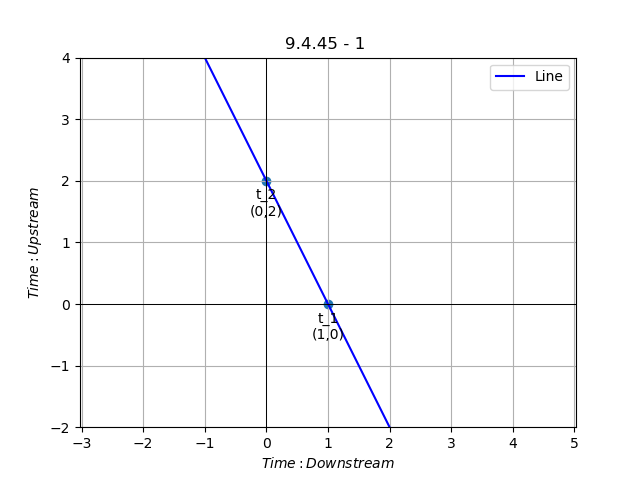
\includegraphics[width=\columnwidth, height=0.8\textheight, keepaspectratio]{../figs/graph1_1.png}   
\end{frame}
 \begin{frame}{Plot}
    \centering
    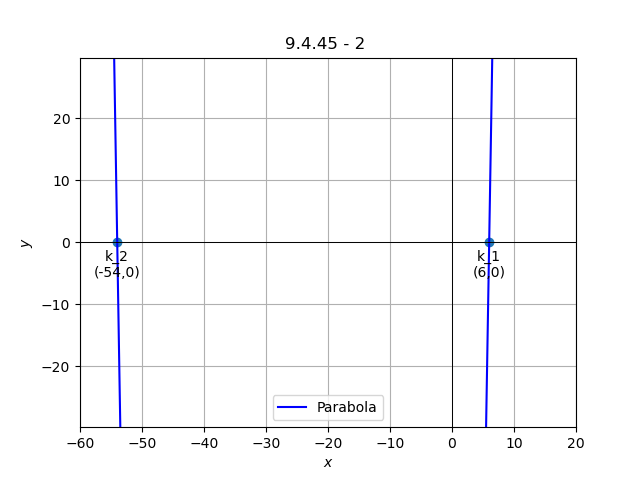
\includegraphics[width=\columnwidth, height=0.8\textheight, keepaspectratio]{../figs/graph1_2.png}   
\end{frame}


\end{document}
